% Contenidos del capítulo.
% Las secciones presentadas son orientativas y no representan
% necesariamente la organización que debe tener este capítulo.

\section{Análisis de aplicaciones similares}
% Qué aplicaciones similares hay y en qué se diferencia de ellas la propuesta

En el contexto de la gestión de casas rurales, así como de las actividades y eventos cercanos a éstas, existen diversas aplicaciones web destacadas que ofrecen funcionalidades avanzadas para la administración y promoción de propiedades. En este apartado se presenta un análisis comparativo de algunas de las plataformas más relevantes, destacando sus principales fortalezas y debilidades.
\subsection{Airbnb}
Airbnb~\cite{airbnb} es una de las aplicaciones de referencia en el sector de alquiler de viviendas y alojamientos turísticos. Esta plataforma ofrece una interfaz amigable y moderna que facilita tanto la búsqueda de propiedades como la gestión de reservas. Además, dispone de herramientas de marketing como la promoción de ofertas y la personalización de sugerencias de viaje, basadas en las preferencias y el historial de los usuarios.

\textbf{Puntos fuertes}:
\begin{itemize}
    \item Interfaz intuitiva y fácil de usar, lo que mejora la experiencia del usuario.
    \item Amplias funcionalidades de recomendación y personalización, adaptadas a los gustos y necesidades de los usuarios.
    \item Sistema de experiencias que permite a los anfitriones ofrecer actividades locales, enriqueciendo la estancia del visitante. La Figura~\ref{fig:airbnb-experiencias} muestra un ejemplo de cómo se presentan estas experiencias en la plataforma.
    \item Integración con múltiples plataformas de pago, aumentando la comodidad para el cliente.
\end{itemize}
\begin{figure}[h!tb]
    \centering
    \setlength{\fboxsep}{15pt}%
    \setlength{\fboxrule}{0.5pt}%
    \fbox{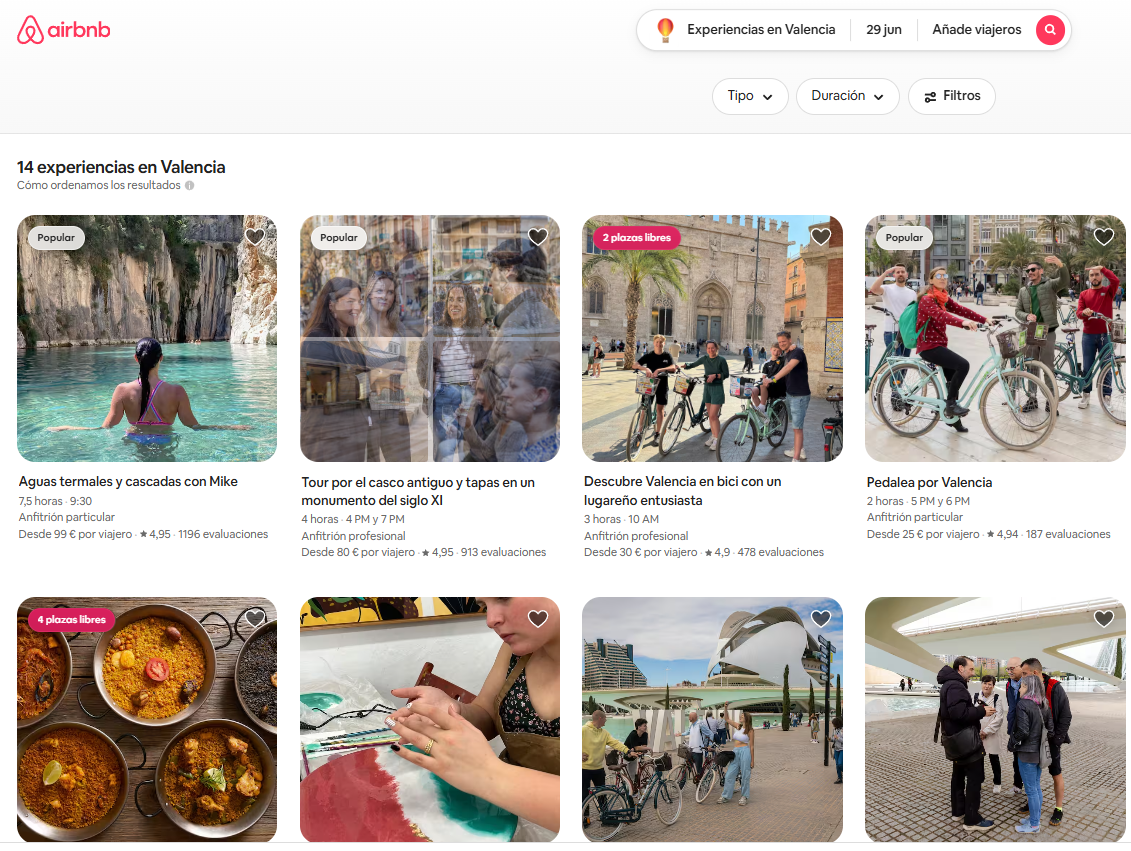
\includegraphics[width=0.9\textwidth]{figs/airbnb_experiencias.png}}
    \caption{Ejemplo de experiencias ofrecidas en Airbnb.}
    \label{fig:airbnb-experiencias}
\end{figure}

\textbf{Puntos débiles}:
\begin{itemize}
    \item Comisiones elevadas para los anfitriones, lo cual puede resultar una desventaja para pequeños propietarios de casas rurales.
    \item Requiere de una conexión constante para la sincronización de datos, lo cual puede no ser óptimo en zonas rurales con cobertura limitada.
    \item Seguridad y privacidad del usuario, ya que existe el riesgo de compartir demasiada información personal en línea.
\end{itemize}

\subsection{Booking.com}
Booking.com~\cite{booking} es otra plataforma ampliamente utilizada para la reserva de alojamientos. Ofrece a los propietarios de casas rurales una plataforma robusta para la gestión de reservas y pagos.

\textbf{Puntos fuertes}:
\begin{itemize}
    \item Amplia visibilidad en el mercado, atrayendo una gran cantidad de usuarios.
    \item Sistema de reseñas con filtros que permiten valorar distintos tipos de experiencia y consultar opiniones relevantes según las fechas deseadas. La Figura~\ref{fig:booking-reviews} muestra un ejemplo de cómo se presentan estas reseñas en la plataforma.
    \item Integración de un sistema de mapas y recomendaciones turísticas locales. La Figura~\ref{fig:booking-mapas} muestra un ejemplo de cómo se presentan estas recomendaciones en la plataforma.
    \item Permite la gestión de propiedades múltiples desde un mismo perfil de anfitrión.
\end{itemize}
\begin{figure}[h!tb]
    \centering
    \setlength{\fboxsep}{15pt}%
    \setlength{\fboxrule}{0.5pt}%
    \fbox{\includegraphics[width=0.9\textwidth]{figs/booking_reseñas.png}}
    \caption{Ejemplo de reseñas en Booking.com.}
    \label{fig:booking-reviews}
\end{figure}
\begin{figure}[h!tb]
    \centering
    \setlength{\fboxsep}{15pt}%
    \setlength{\fboxrule}{0.5pt}%
    \fbox{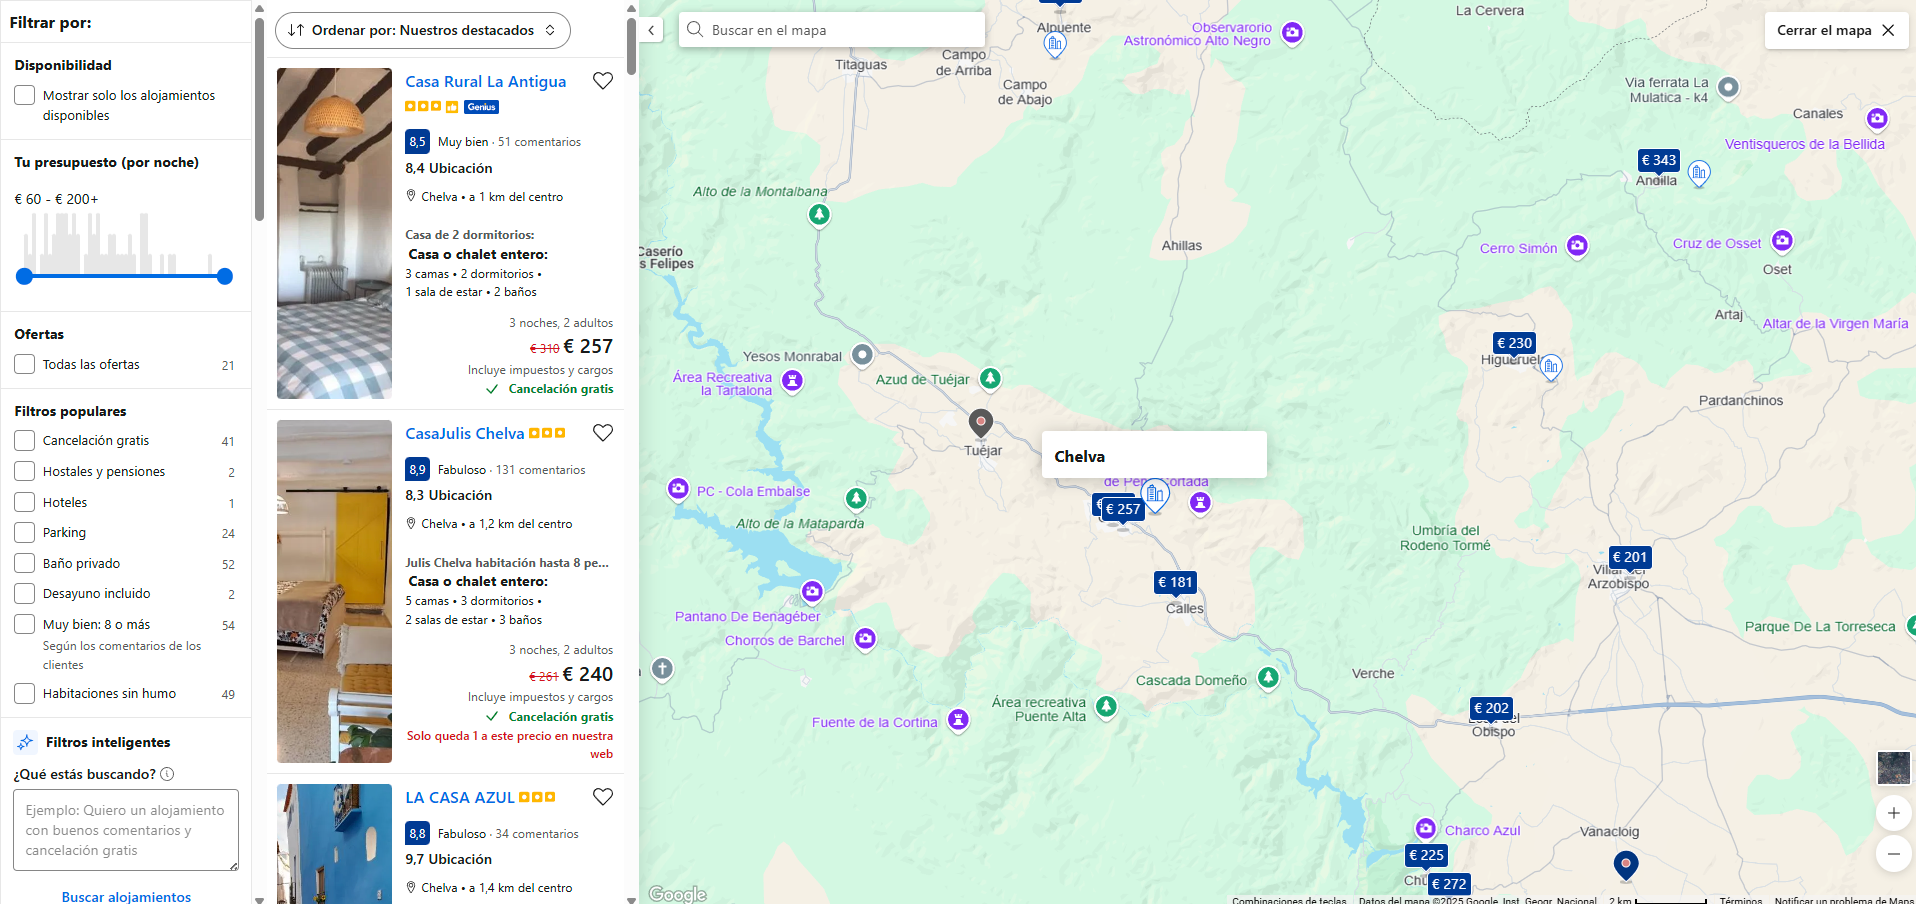
\includegraphics[width=0.9\textwidth]{figs/booking.png}}
    \caption{Ejemplo de recomendaciones turísticas en Booking.com.}
    \label{fig:booking-mapas}
\end{figure}

\textbf{Puntos débiles}:
\begin{itemize}
    \item Costos de servicio elevados y comisiones en cada reserva.
    \item Dificultades en la personalización de la experiencia del usuario, limitando las opciones de personalización para el anfitrión.
    \item Falta de opciones de promoción específicas para propietarios de casas rurales, comparado con otras plataformas.
\end{itemize}

\subsection{Ruralka}
Ruralka~\cite{ruralka} es una plataforma específica para el alquiler de casas rurales en España, enfocada en ofrecer experiencias únicas en entornos naturales.

\textbf{Puntos fuertes}:
\begin{itemize}
    \item Enfoque en la experiencia rural, destacando actividades al aire libre y experiencias culturales personalizadas por el anfitrión.
    \item Sistema sencillo de servicios adaptado a la experiencia buscada en casas rurales. La Figura~\ref{fig:ruralka-servicios} muestra un ejemplo de cómo se presentan estos servicios en la plataforma.
    \item Selección cuidada de propiedades que garantiza una calidad estandarizada.
    \item Proporciona una mayor visibilidad a pequeños propietarios rurales, con tarifas de servicio más bajas en comparación con plataformas generalistas.
\end{itemize}

\begin{figure}[h!tb]
    \centering
    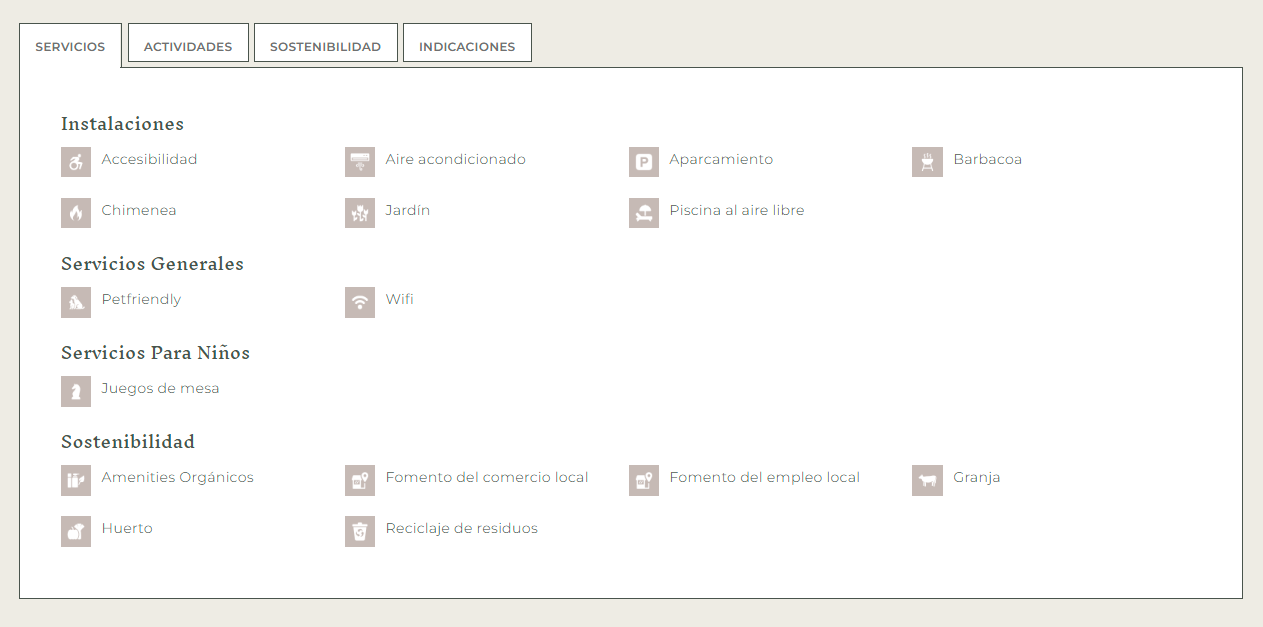
\includegraphics[width=1\textwidth]{figs/ruralka_servicios.png}
    \caption{Ejemplo de servicios ofrecidos en Ruralka.}
    \label{fig:ruralka-servicios}
\end{figure}

\textbf{Puntos débiles}:
\begin{itemize}
    \item Menor alcance en términos de tráfico y usuarios comparado con grandes plataformas internacionales.
    \item Limitación en opciones de pago y personalización de propiedades, lo cual puede ser un inconveniente para algunos usuarios.
\end{itemize}
\subsection{Komoot}
Komoot~\cite{komoot} es una plataforma especializada en la planificación y descubrimiento de rutas para actividades al aire libre como senderismo, ciclismo, running o excursiones en la naturaleza. Se ha consolidado como una de las aplicaciones más utilizadas en Europa para explorar rutas personalizadas y obtener recomendaciones según el nivel de dificultad, el tipo de terreno o el paisaje.

\textbf{Puntos fuertes}:
\begin{itemize}
\item Amplia base de datos de rutas, mapas y puntos de interés generados por la comunidad de usuarios.
\item Posibilidad de personalizar rutas según actividad, condición física y tipo de terreno. Esto se puede observar en la Figura~\ref{fig:komoot-rutas}, donde se muestran ejemplos de rutas personalizadas y cómo podemos planificarlas.            
\item Navegación guiada por voz incluso sin conexión a Internet, ideal para zonas rurales con cobertura limitada.
\item Integración con relojes GPS y dispositivos de ciclismo para registrar y compartir rutas.
\end{itemize}

\begin{figure}[h!tb]
    \centering
    \setlength{\fboxsep}{15pt}%
    \setlength{\fboxrule}{0.5pt}%
    \fbox{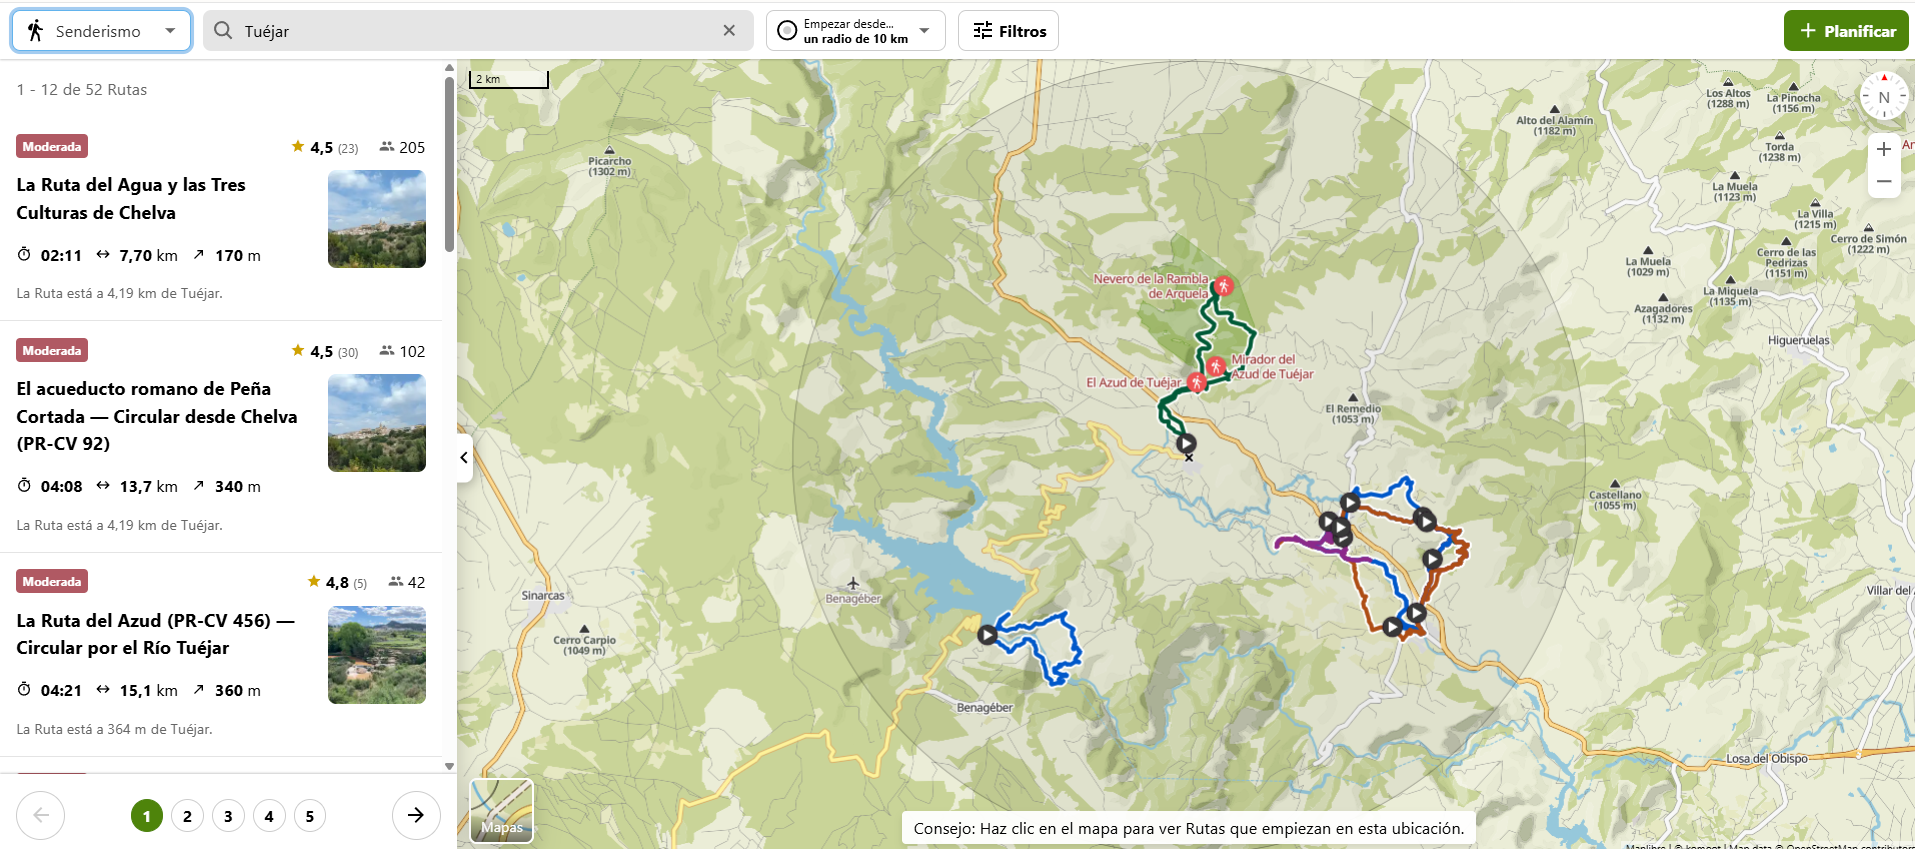
\includegraphics[width=0.9\textwidth]{figs/koomot.png}}
    \caption{Ejemplo de rutas personalizadas en Komoot.}
    \label{fig:komoot-rutas}        
\end{figure}

\textbf{Puntos débiles}:
\begin{itemize}
\item Algunas funcionalidades avanzadas requieren suscripción de pago (por ejemplo, mapas detallados offline por región).
\item Interfaz menos atractiva en comparación con otras aplicaciones de planificación de viajes.
\item Menor presencia en países no europeos, lo que puede limitar la oferta de rutas si la casa rural se encuentra en una región menos explorada por la comunidad.
\end{itemize}

Este análisis de aplicaciones muestra tanto las oportunidades como los desafíos que estas plataformas enfrentan en el mercado actual. Nuestra aplicación de gestión y marketing para una casa rural busca combinar las mejores prácticas de estas plataformas —alojamiento, actividades al aire libre y eventos culturales— y adaptarlas en una solución integral que facilite tanto la visibilidad del alojamiento como la promoción de experiencias completas. Al ofrecer una gestión automatizada y sin necesidad de conocimientos técnicos, se potencia la autonomía del propietario y se mejora la experiencia del visitante desde el descubrimiento hasta la participación en actividades locales.

\section{APIs y plataformas externas a utilizar}

Para el correcto funcionamiento del sistema de gestión de la casa rural, se integrarán diversas \glspl{API} y plataformas externas. Estas fuentes permitirán extraer información turística, contenidos multimedia y datos meteorológicos relevantes para enriquecer la experiencia del usuario. A continuación, se detallan las principales herramientas seleccionadas, su funcionalidad y un análisis de sus ventajas e inconvenientes.

\subsection{Portal turístico de Tuéjar}
El portal turístico oficial de Tuéjar~\cite{url.tuejar} ofrece información actualizada sobre rutas, actividades y patrimonio natural y cultural del municipio. Este sitio se utilizará como fuente para el raspado automático de contenidos relacionados con eventos locales y lugares de interés. En la Figura~\ref{fig:tuejar-web} se muestra un ejemplo de cómo se presenta la información turística en la web de Tuéjar.

\textbf{Puntos fuertes}:
\begin{itemize}
    \item Información específica y localizada sobre el entorno rural.
    \item Actualización frecuente de eventos locales y propuestas turísticas.
    \item Fuente confiable y mantenida por el ayuntamiento o entes locales.
\end{itemize}

\textbf{Puntos débiles}:
\begin{itemize}
    \item Estructura web variable que puede dificultar la automatización del raspado.
    \item Falta de API oficial, lo que obliga a depender del web scraping.
\end{itemize}

\begin{figure}[h!tb]
    \centering
    \setlength{\fboxsep}{15pt}%
    \setlength{\fboxrule}{0.5pt}%
    \fbox{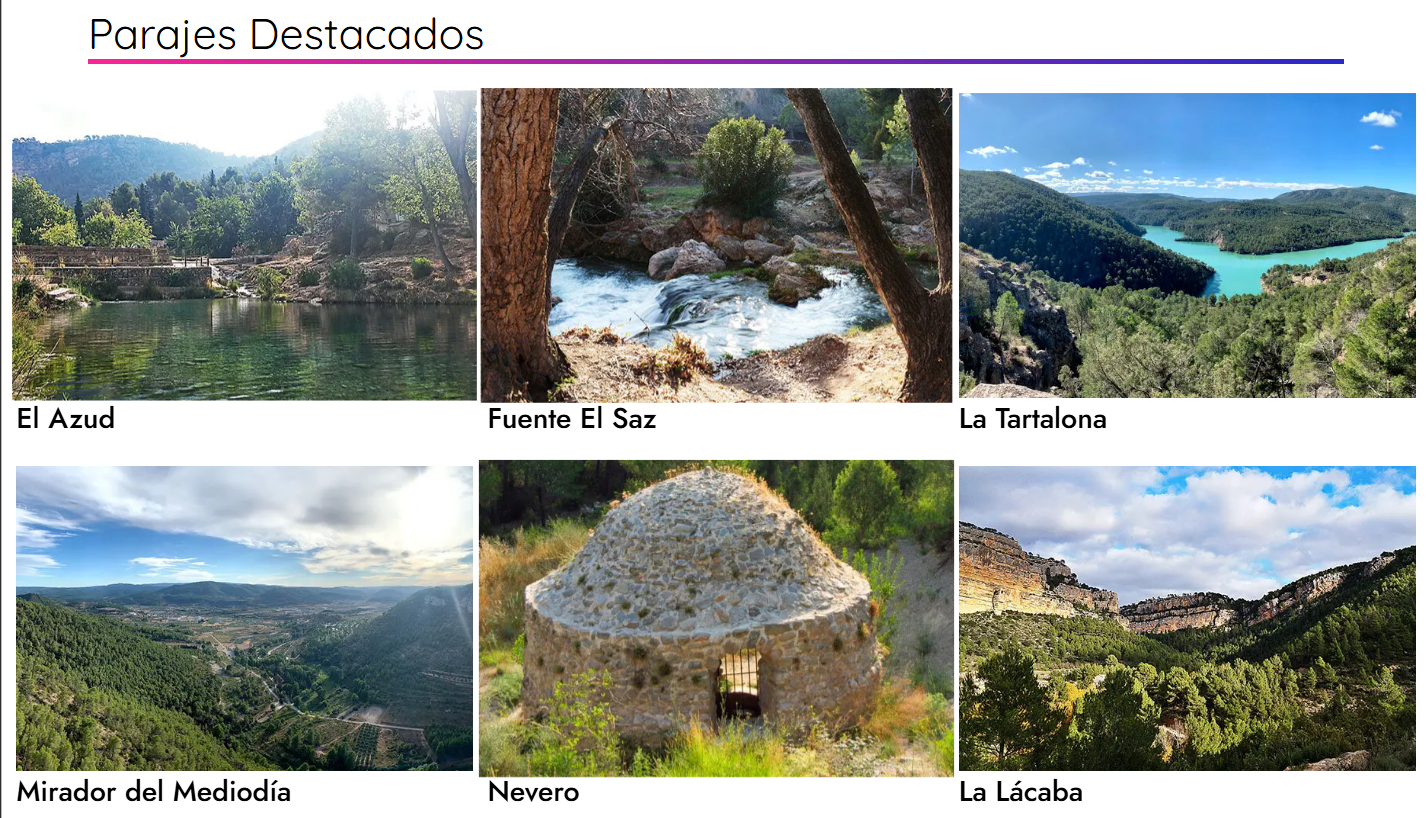
\includegraphics[width=0.9\textwidth]{figs/tuejar_turismo.png}}
    \caption{Ejemplo de información turística extraída de la web de Tuéjar.}
    \label{fig:tuejar-web}
\end{figure}

\subsection{Portal turístico de Chelva}
El sitio web de turismo de Chelva~\cite{url.chelva} se utilizará como fuente secundaria para obtener eventos, fiestas populares, rutas y otras actividades cercanas a Tuéjar. El objetivo es ampliar el abanico de recomendaciones disponibles para los visitantes. 
En la Figura~\ref{fig:chelva-web} se muestra un ejemplo de cómo se presentan y están accesibles de forma sencilla monumentos, espacios naturales, aldeas y fiestas en la web de Chelva.

\textbf{Puntos fuertes}:
\begin{itemize}
    \item Información turística de un municipio cercano, complementaria a la de Tuéjar.
    \item Contenido visual útil para la promoción de actividades (imágenes, carteles de eventos, etc.).
\end{itemize}

\textbf{Puntos débiles}:
\begin{itemize}
    \item Dificultad de estructuración para el raspado, ya que su diseño web no sigue patrones estándar.
    \item Contenido limitado a eventos puntuales.
\end{itemize}

\begin{figure}[h!tb]
    \centering
    \setlength{\fboxsep}{15pt}%
    \setlength{\fboxrule}{0.5pt}%
    \fbox{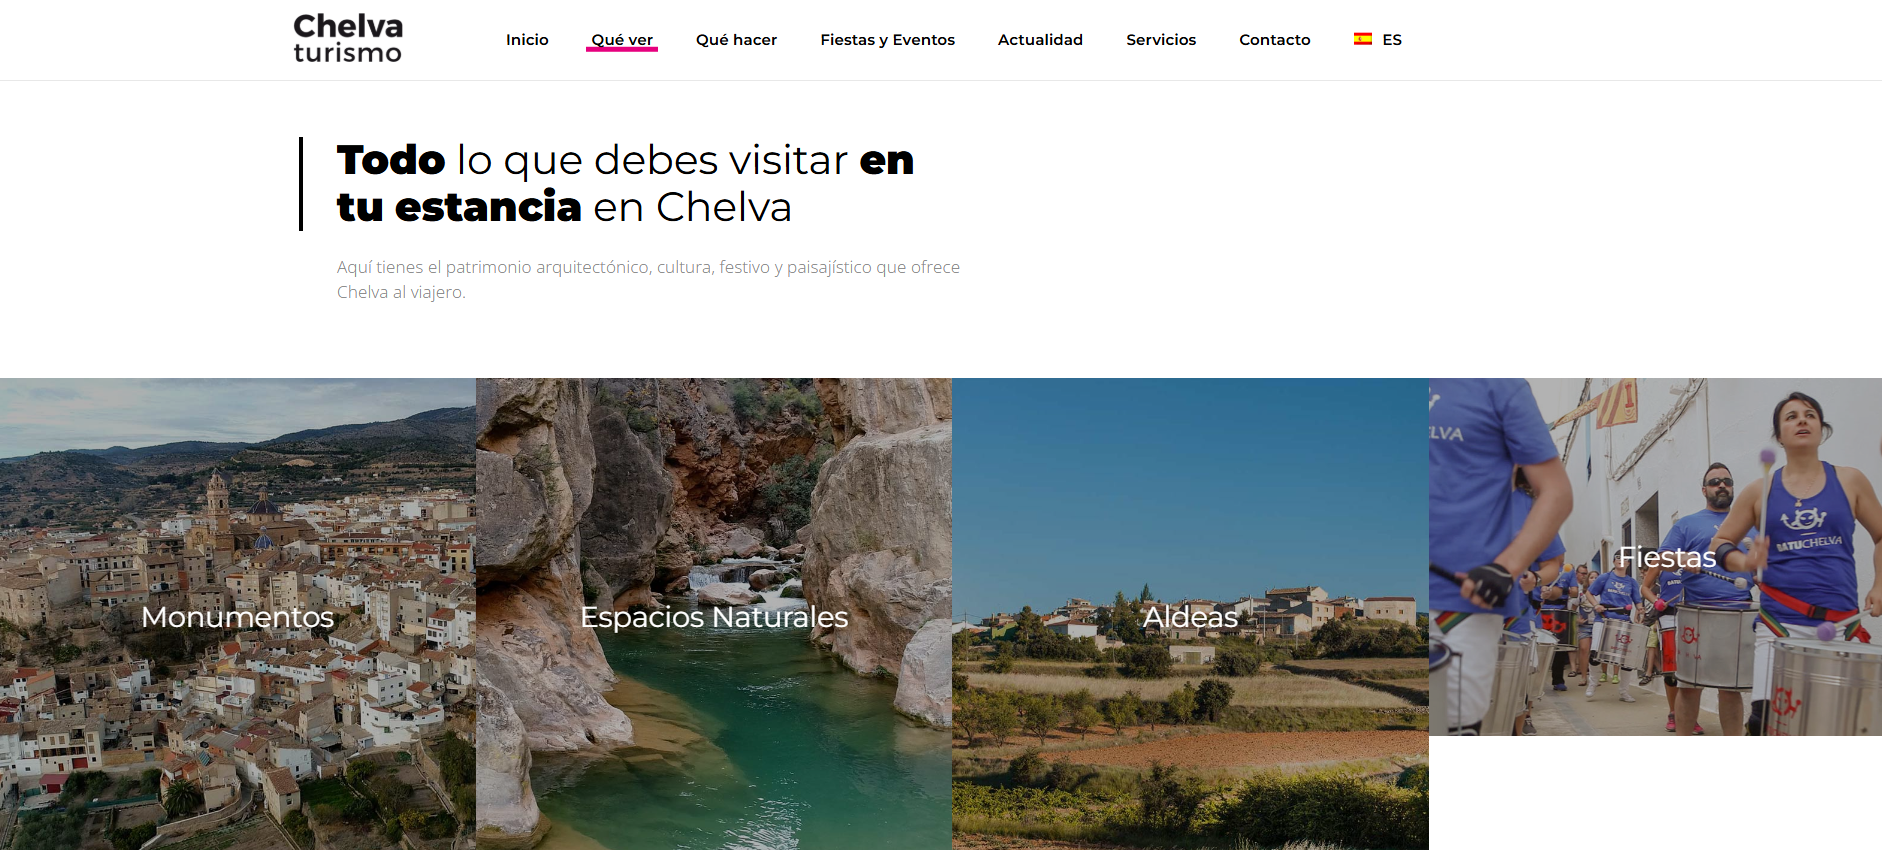
\includegraphics[width=0.9\textwidth]{figs/chelva_turismo.png}}
    \caption{Ejemplo de rutas y eventos extraídos de la web de turismo de Chelva.}
    \label{fig:chelva-web}
\end{figure}

\subsection{Web oficial del Ayuntamiento de Tuéjar}
La web institucional del Ayuntamiento~\cite{url.aytuejar} contiene convocatorias, noticias municipales y eventos oficiales que pueden ser relevantes para los usuarios de la plataforma, especialmente en el contexto de fiestas patronales o ferias. Como se observa en la Figura~\ref{fig:ayto-web}, la web del Ayuntamiento de Tuéjar ofrece información sobre eventos locales y festividades de las cuales extraer los recursos para la plataforma. 

\textbf{Puntos fuertes}:
\begin{itemize}
    \item Información oficial y validada por el consistorio.
    \item Acceso a contenido de interés general para residentes y visitantes.
\end{itemize}

\textbf{Puntos débiles}:
\begin{itemize}
    \item Página orientada a trámites administrativos, no siempre con contenido turístico directo.
    \item Variabilidad en la estructura del contenido que complica el scraping sistemático.
\end{itemize}

\begin{figure}[h!tb]
    \centering
    \setlength{\fboxsep}{15pt}%
    \setlength{\fboxrule}{0.5pt}%
    \fbox{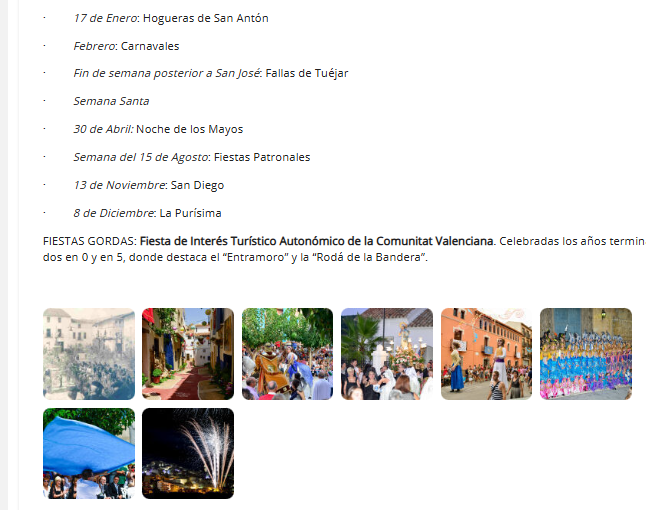
\includegraphics[width=0.9\textwidth]{figs/ayuntamiento_tuejar.png}}
    \caption{Contenido institucional relevante en la web del Ayuntamiento de Tuéjar.}
    \label{fig:ayto-web}
\end{figure}

\subsection{API de Instagram Graph}
La \textit{Instagram Graph API}~\cite{instagram-graph-api} permitirá obtener publicaciones relacionadas con la casa rural, eventos locales y fotografías etiquetadas en la zona. Será utilizada para enriquecer la sección multimedia de la plataforma, conectando contenido generado por el gestor sobre su perfil de Instagram.

\textbf{Puntos fuertes}:
\begin{itemize}
    \item Acceso a publicaciones recientes mediante hashtags o localizaciones.
    \item Contenido auténtico y visual, generado por el gestor.
    \item Posibilidad de integración con galerías dinámicas en la plataforma.
\end{itemize}

\textbf{Puntos débiles}:
\begin{itemize}
    \item Requiere autenticación y permisos para acceder a ciertos datos.
    \item Cambios frecuentes en las políticas de uso y limitaciones en las llamadas a la API.
\end{itemize}



\subsection{API meteorológica Open-Meteo}
La \textbf{\gls{API} de Open-Meteo}~\cite{open-meteo-api} será la fuente principal para obtener datos meteorológicos en la plataforma. Esta \gls{API} pública ofrece información precisa y en tiempo real, sin necesidad de autenticación mediante token, lo que simplifica su integración y uso en aplicaciones automatizadas.

\textbf{Puntos fuertes}:
\begin{itemize}
    \item No requiere tokenización ni registro, facilitando el acceso directo a los datos.
    \item Permite obtener datos históricos de predicción, lo que posibilita aplicar modelos propios para prever condiciones futuras en función de patrones pasados.
    \item Proporciona estimaciones muy precisas basadas en modelos meteorológicos de última generación y ajustadas a la ubicación exacta mediante coordenadas geográficas.
    \item Respuesta en formato JSON clara y fácilmente integrable con el sistema.
\end{itemize}

\textbf{Puntos débiles}:
\begin{itemize}
    \item Aunque ofrece predicciones detalladas, no incluye avisos oficiales sobre fenómenos adversos como lo hace AEMET.
\end{itemize}


\subsection{API meteorológica AEMET}
La \gls{API} de \gls{aemet}~\cite{aemet-api} fue evaluada como posible alternativa, ya que proporciona datos oficiales en el ámbito nacional. Sin embargo, se descartó como fuente principal por las siguientes razones:

\begin{itemize}
    \item La ubicación de la casa rural no cuenta con una estación meteorológica de \gls{aemet} cercana, por lo que los datos disponibles son menos representativos de las condiciones reales.
    \item Requiere autenticación mediante token y tiene limitaciones de uso que complican su automatización continua.
\end{itemize}


\section{Evaluación de tecnologías}
\label{sec:evaluacion-tecnologias}
Para el desarrollo de aplicaciones web, existen múltiples tecnologías, \glspl{framework} y bases de datos disponibles. A continuación, se describen algunas de las alternativas más comunes, destacando sus características y diferencias. Finalmente, se justifica la elección de Angular~\cite{angular}, Spring Boot~\cite{springboot}, Docker~\cite{docker} y \gls{k8s}~\cite{kubernetes} como las herramientas de desarrollo principales para está aplicación, junto con el uso de distintas bases de datos adaptadas a cada caso de uso que se detallará más adelante. La principal motivación para elegir estas tecnologías es continuar y profundizar en los conocimientos adquiridos en el programa del máster.


\subsection{\gls{frontend}}

\paragraph{Angular~\cite{angular}} es un \gls{framework} de desarrollo de aplicaciones web de Google basado en \gls{typescript}, que permite construir interfaces de usuario dinámicas y altamente interactivas. Comparado con otras tecnologías como React o Vue.js, Angular ofrece un ecosistema completo que incluye enrutamiento, inyección de dependencias y herramientas de pruebas.

\textbf{Ventajas}:
\begin{itemize}
    \item Arquitectura robusta basada en componentes y módulos.
    \item Excelente rendimiento y herramientas para el desarrollo de aplicaciones a gran escala.
    \item Comunidad activa y soporte continuo de Google.
\end{itemize}

\textbf{Desventajas}:
\begin{itemize}
    \item Curva de aprendizaje pronunciada debido a su estructura compleja.
    \item Tamaño relativamente grande del \gls{framework} en comparación con alternativas como Vue.js.
\end{itemize}

\paragraph{React~\cite{react}} es una biblioteca de \gls{javascript} desarrollada por \gls{meta}, centrada en la construcción de interfaces de usuario a través de componentes. A diferencia de Angular, React es una biblioteca más ligera y flexible, aunque se requiere la integración de herramientas adicionales para lograr funcionalidades completas.

\textbf{Ventajas}:
\begin{itemize}
    \item Flexibilidad para integrarse con otras bibliotecas y herramientas.
    \item Alta velocidad de renderizado gracias al uso de un DOM virtual.
    \item Gran popularidad y extensa comunidad, con abundante documentación y recursos.
\end{itemize}

\textbf{Desventajas}:
\begin{itemize}
    \item Mayor necesidad de configuración e integración de herramientas externas (por ejemplo, enrutamiento y gestión de estado).
    \item La flexibilidad y falta de estructura puede resultar confusa para proyectos grandes.
\end{itemize}
\textbf{Conclusión:} Tanto Angular como React representan soluciones sólidas para el desarrollo de interfaces web modernas, pero con enfoques y características claramente diferenciadas. Angular ofrece un ecosistema integral ideal para aplicaciones empresariales de gran escala, aunque su complejidad inicial puede suponer una barrera. React, en cambio, destaca por su flexibilidad y rendimiento, siendo una opción preferida cuando se busca una solución más ligera y adaptable. En el contexto del presente \gls{tfm}, se ha optado por Angular debido a su amplia utilización a lo largo del desarrollo, su arquitectura robusta y la facilidad para integrar funcionalidades avanzadas sin depender de bibliotecas externas.

\subsection{Backend}

\paragraph{Spring Boot~\cite{springboot}} es un marco de trabajo para el desarrollo de aplicaciones \gls{backend} en Java. A diferencia de alternativas como Express (Node.js) o Django (Python), Spring Boot permite crear microservicios escalables y altamente configurables.

\textbf{Ventajas}:
\begin{itemize}
    \item Gran capacidad de integración con sistemas empresariales.
    \item Alto rendimiento en aplicaciones de gran escala y fácil escalabilidad.
    \item Amplio ecosistema de herramientas y bibliotecas, como Spring Data para la gestión de bases de datos y Spring Security para la autenticación y autorización.
    \item Amplio soporte para programación reactiva~\cite{hashemi2025reactive} y arquitectura de microservicios. Esto permitirá la utilización de extensiones como Spring WebFlux~\cite{webflux} para construir aplicaciones reactivas y eficientes.
\end{itemize}

\textbf{Desventajas}:
\begin{itemize}
    \item Consumo de memoria elevado, lo cual puede ser un inconveniente en aplicaciones de recursos limitados.
    \item Complejidad en la configuración inicial, especialmente para desarrolladores principiantes.
\end{itemize}


\paragraph{Django~\cite{django}} es un \gls{framework} de desarrollo web en Python que permite construir aplicaciones web de manera rápida y eficiente, utilizando una arquitectura basada en el patrón \gls{mvc}. A diferencia de otros \glspl{framework} como Flask\cite{flask} (Python) o Express (Node.js), Django proporciona una gran cantidad de herramientas y componentes listos para usar, facilitando el desarrollo de aplicaciones complejas.

\textbf{Ventajas}: \begin{itemize} \item Gran cantidad de funcionalidades integradas, incluyendo autenticación, administración y protección contra ataques comunes, lo que acelera el desarrollo. \item Arquitectura escalable y organizada, ideal para aplicaciones de mediana y gran escala. \item Genera aplicaciónes \gls{spa}~\cite{fenollosa2022spa} \item Fuerte comunidad de soporte y documentación exhaustiva, que facilita la resolución de problemas y el aprendizaje. \end{itemize}

\textbf{Desventajas}: \begin{itemize} \item Puede ser excesivo para aplicaciones pequeñas o simples, debido a su estructura robusta. \item Curva de aprendizaje para aquellos que no están familiarizados con Python o con el enfoque MVC de Django. \item Limitaciones en la personalización de ciertas partes del \gls{framework}, lo cual puede ser un inconveniente en proyectos altamente específicos. \end{itemize}

\paragraph{Express(Node.js)~\cite{express}} es un \gls{framework} minimalista para Node.js que permite desarrollar aplicaciones \gls{backend} con \gls{javascript} o TypeScript. Su simplicidad y capacidad para construir \glspl{API} \gls{rest} lo hacen ideal para aplicaciones pequeñas y medianas.

\textbf{Ventajas}:
\begin{itemize}
    \item Ligero y rápido, ideal para aplicaciones que requieren una alta velocidad de respuesta.
    \item Ecosistema de módulos y paquetes que facilita la ampliación de funcionalidades.
    \item Compatibilidad total con \gls{javascript} en el \gls{frontend}, lo que permite un desarrollo \gls{fullstack} unificado.
\end{itemize}

\textbf{Desventajas}:
\begin{itemize}
    \item No ofrece tantas funcionalidades integradas como \glspl{framework} más robustos como Spring Boot, lo cual requiere el uso de bibliotecas adicionales.
    \item Menor rendimiento en aplicaciones de alta carga comparado con alternativas basadas en Java.
\end{itemize}
\textbf{Conclusión:} Spring Boot, Django y Express representan enfoques distintos para el desarrollo de aplicaciones \gls{backend}, cada uno con sus propias ventajas. Spring Boot ofrece una solución completa y altamente escalable, ideal para entornos empresariales, aunque con un mayor consumo de recursos. Django destaca por su rapidez de desarrollo y funcionalidades integradas, mientras que Express se orienta a proyectos ligeros y rápidos gracias a su simplicidad. En el presente \gls{tfm}, se ha optado por Spring Boot debido a su amplia utilización durante el desarrollo del proyecto, su integración nativa con herramientas empresariales y su compatibilidad con una arquitectura basada en microservicios reactivos.

\subsection{Contenerización y Orquestación}

\paragraph{Docker~\cite{docker}} es una tecnología de contenedorización que permite empaquetar aplicaciones y sus dependencias en contenedores ligeros, portables y aislados. Gracias a su amplio ecosistema y facilidad de uso, se ha convertido en el estándar de facto en entornos de desarrollo y despliegue moderno. A diferencia de soluciones como LXC~\cite{lxc}, Docker proporciona una capa de abstracción más amigable al desarrollador, centrada en la construcción y distribución de aplicaciones mediante imágenes reutilizables.

\textbf{Ventajas}:
\begin{itemize}
    \item Portabilidad entre distintos entornos gracias al empaquetado en imágenes.
    \item Rapidez en el despliegue y facilidad para replicar entornos.
    \item Amplia comunidad y disponibilidad de herramientas complementarias.
\end{itemize}

\textbf{Desventajas}:
\begin{itemize}
    \item Puede consumir más recursos que soluciones de virtualización más ligeras como LXC.
    \item Requiere una adecuada configuración de seguridad para entornos de producción.
\end{itemize}

\paragraph{Kubernetes~\cite{kubernetes}} (o \gls{k8s}) es una plataforma de orquestación de contenedores que automatiza el despliegue, escalado y gestión de aplicaciones en contenedores. Se integra comúnmente con Docker como motor de contenedores, aunque también soporta otras alternativas. En comparación con soluciones más simples como Docker Swarm~\cite{dockerswarm}, Kubernetes ofrece un mayor control sobre redes, almacenamiento y políticas de autosanación.

\textbf{Ventajas}:
\begin{itemize}
    \item Escalabilidad horizontal y alta disponibilidad mediante replicación automática.
    \item Orquestación avanzada con balanceo de carga, monitoreo y autoescalado.
    \item Gran ecosistema y soporte por parte de los principales proveedores cloud.
\end{itemize}

\textbf{Desventajas}:
\begin{itemize}
    \item Curva de aprendizaje elevada debido a su complejidad.
    \item Requiere mayor inversión en infraestructura y conocimientos técnicos.
\end{itemize}

\paragraph{LXC (Linux Containers)~\cite{lxc}} es una tecnología de virtualización a nivel de sistema operativo que permite ejecutar múltiples entornos Linux aislados dentro de un mismo kernel. A diferencia de Docker, que opera a un nivel más alto centrado en las aplicaciones, LXC ofrece un control más detallado sobre el entorno del sistema, siendo más parecido a una máquina virtual ligera.

\textbf{Ventajas}:
\begin{itemize}
    \item Mayor control sobre los procesos y el entorno del sistema operativo.
    \item Menor sobrecarga de recursos al compartir el mismo kernel del host.
\end{itemize}

\textbf{Desventajas}:
\begin{itemize}
    \item Menor facilidad de uso y adopción en comparación con Docker.
    \item Integración limitada con herramientas modernas de orquestación como \gls{k8s}.
\end{itemize}

\paragraph{Docker Swarm~\cite{dockerswarm}} es la solución de orquestación nativa de Docker, diseñada para desplegar y gestionar clústeres de contenedores de forma más simple que Kubernetes. Aunque ofrece una integración fluida con el ecosistema Docker, su uso ha disminuido frente al crecimiento y madurez de \gls{k8s}.

\textbf{Ventajas}:
\begin{itemize}
    \item Sencillez de configuración y despliegue en comparación con Kubernetes.
    \item Integración directa con Docker CLI y Docker Compose.
\end{itemize}

\textbf{Desventajas}:
\begin{itemize}
    \item Menor escalabilidad y robustez en entornos de producción complejos.
    \item Comunidad y soporte más reducidos, con menor ritmo de desarrollo.
\end{itemize}
\textbf{Conclusión:} Las tecnologías de contenedorización y orquestación han revolucionado el despliegue y la gestión de aplicaciones. Docker se ha consolidado como una solución estándar por su facilidad de uso, portabilidad y amplio soporte. Kubernetes, por su parte, representa la opción más robusta para orquestar contenedores a gran escala, ofreciendo funcionalidades avanzadas de escalabilidad y resiliencia. Frente a alternativas como LXC o Docker Swarm, ambas herramientas destacan por su madurez y adopción en entornos productivos. En el presente \gls{tfm}, se han elegido Docker y Kubernetes debido a su amplia utilización durante el desarrollo, así como a su integración fluida y capacidad para soportar arquitecturas distribuidas y escalables en la nube.
\subsection{Bases de Datos}

Para el desarrollo de la aplicación, es necesario almacenar datos en diferentes tipos de bases de datos, según el caso de uso específico. A continuación, se analizan las bases de datos NoSQL, destinadas al almacenamiento de contenido multimedia etiquetado; las bases de datos SQL, utilizadas para la gestión de autenticación y reservas; y las bases de datos en memoria, implementadas para optimizar el rendimiento en el acceso a datos temporales o frecuentemente consultados. Cabe destacar que todas las bases de datos comparadas son compatibles o tienen equivalencias con servicios de plataforma en la nube, tanto a nivel de \gls{iaas} como de \gls{paas}, los cuales se compararán en el apartado siguiente.

\paragraph{Bases de datos NoSQL}
Para almacenar contenido multimedia y etiquetas de categorización, se evaluarán MongoDB y Cassandra.

\textbf{MongoDB~\cite{mongodb}} es una base de datos orientada a documentos que almacena datos en formato BSON, ideal para aplicaciones que requieren flexibilidad en el esquema y escalabilidad horizontal.

\textbf{Ventajas}:
\begin{itemize}
\item Modelo de datos flexible y basado en documentos, ideal para almacenar contenido multimedia y metadatos asociados.
\item Facilidad para realizar consultas complejas en estructuras de datos anidadas.
\item Escalabilidad horizontal, con soporte nativo para fragmentación de datos.
\end{itemize}

\textbf{Desventajas}:
\begin{itemize}
\item Mayor consumo de memoria y almacenamiento.
\item Rendimiento limitado en consultas a gran escala comparado con Cassandra.
\end{itemize}

\textbf{Cassandra~\cite{cassandra}} es una base de datos distribuida orientada a columnas, diseñada para manejar grandes volúmenes de datos en múltiples nodos, ideal para aplicaciones de alta disponibilidad.

\textbf{Ventajas}:
\begin{itemize}
\item Escalabilidad masiva y resistencia a fallos, gracias a su arquitectura distribuida.
\item Alta eficiencia en escritura y lectura de grandes cantidades de datos.
\end{itemize}

\textbf{Desventajas}:
\begin{itemize}
\item Curva de aprendizaje y configuración compleja.
\item Menor flexibilidad en la estructura de datos en comparación con MongoDB.
\end{itemize}

\textbf{Conclusión:} En este proyecto, MongoDB resulta ser la elección más apropiada para almacenar contenido multimedia con etiquetas, debido a su flexibilidad.

\paragraph{Bases de datos SQL}
Para la gestión de autenticación y reservas, se evaluarán PostgreSQL~\cite{postgresql} y MySQL~\cite{mysql}, así como Oracle~\cite{oracle} y MariaDB~\cite{mariadb}.

\textbf{PostgreSQL~\cite{postgresql}} es una base de datos relacional con soporte avanzado de SQL y capacidades de extensibilidad.

\textbf{Ventajas}:
\begin{itemize}
\item Potente soporte para operaciones complejas y consultas avanzadas.
\item Extensible y con un sólido soporte de integridad referencial y transacciones.
\end{itemize}

\textbf{MySQL~\cite{mysql}} es una base de datos relacional conocida por su simplicidad y eficiencia en el procesamiento de transacciones de lectura-escritura.

\textbf{Ventajas}:
\begin{itemize}
\item Amplia compatibilidad y facilidad de uso.
\item Buen rendimiento para aplicaciones de lectura intensiva.
\end{itemize}

\textbf{Oracle~\cite{oracle}} es una base de datos relacional empresarial, con características avanzadas orientadas a entornos críticos y escalables.

\textbf{Ventajas}:
\begin{itemize}
\item Gran capacidad para gestión de grandes volúmenes de datos y alta concurrencia.
\item Funcionalidades avanzadas de seguridad y replicación.
\end{itemize}

\textbf{MariaDB~\cite{mariadb}} es un fork de MySQL que ofrece mejoras en rendimiento y nuevas características manteniendo compatibilidad.

\textbf{Ventajas}:
\begin{itemize}
\item Mejoras en rendimiento y en almacenamiento en comparación con MySQL.
\item Comunidad activa y desarrollo abierto.
\end{itemize}

\textbf{Conclusión:} Tanto PostgreSQL como MySQL cumplen con los requisitos de tablas sencillas para la gestión de autenticación y reservas, por lo que se puede optar por cualquiera. Además, la selección de estas bases de datos se ha realizado también pensando en el entorno de desarrollo backend utilizado durante el máster, donde se estudió la integración principalmente con PostgreSQL y MySQL, facilitando así la compatibilidad y el soporte durante el desarrollo. Por este motivo, Oracle y MariaDB, aunque válidas, no fueron seleccionadas para este proyecto.

\paragraph{Bases de datos en memoria}
Para mejorar el rendimiento en el acceso a datos temporales o frecuentemente consultados, se consideran bases de datos en memoria. Aquí se compararán Redis y Memcached.

\textbf{Redis~\cite{redis}} es una base de datos en memoria basada en un modelo de estructura de datos clave-valor con soporte para varios tipos de estructuras de datos.

\textbf{Ventajas}:
\begin{itemize}
\item Alta velocidad de acceso a datos.
\item Soporte para estructuras de datos complejas y persistencia opcional.
\end{itemize}

\textbf{Memcached~\cite{memcached}} es una solución de almacenamiento en caché distribuido que también utiliza un modelo clave-valor, optimizado para operaciones de lectura y escritura de alta velocidad.

\textbf{Ventajas}:
\begin{itemize}
\item Rápido y ligero, ideal para almacenamiento en caché simple.
\end{itemize}

\textbf{Conclusión:} Redis es la opción preferida en este proyecto para datos en memoria, gracias a su soporte para estructuras complejas y manejo eficiente de datos temporales. Además, de ser una herramienta utilizada durante el desarrollo del máster.

\subsection{Servicios de plataformas en la nube}

A la hora de desplegar aplicaciones web, existen diferentes proveedores de plataformas en la nube que ofrecen servicios variados dependiendo de las necesidades de escalabilidad, rendimiento y costos. A continuación, en la Tabla~\ref{tbl:comparacion_plataformas} se presenta una comparación entre los principales proveedores para ayudarte a elegir la opción más adecuada para el despliegue de tu aplicación.


\begin{table}[h!tb] 
    \centering
    \resizebox{\textwidth}{!}{ 
    \begin{tabular}{|c|c|c|c|c|c|c|c|c|} 
    \hline
    \textbf{Plataforma} & \textbf{Servicio gratuito} & \textbf{Dominio Gratis} & \textbf{Frontend} & \textbf{Backend} & \textbf{Base de datos} & \textbf{Kubernetes} \\
    \hline
    AWS     & No & No & Sí & Sí & Sí & Sí \\
    \hline
    GCP     & No & No & Sí & Sí & Sí & Sí \\
    \hline
    Azure   & No & No & Sí & Sí & Sí & Sí \\
    \hline
    Vercel  & Sí para uso básico & Sí (\texttt{vercel.app}) & Sí & No & No & No \\
    \hline
    Netlify & Sí para uso básico & Sí (\texttt{netlify.app}) & Sí & No & No & No \\
    \hline
    Render  & Sí para uso básico & No & Sí & Sí & Sí(limitado) & No \\
    \hline
    Firebase & Sí para uso básico & Sí (\texttt{firebaseapp.com}) & No & No & Sí & No \\
    \hline
    \end{tabular}
    }
    \caption{Comparación de Plataformas para Despliegue de Aplicaciones}
    \label{tbl:comparacion_plataformas}
\end{table}


\subsubsection*{Descripción de los servicios}


\begin{itemize}
    \item \textbf{\gls{aws}\cite{aws-ref}}: \gls{aws} ofrece una amplia variedad de servicios, incluyendo instancias \gls{ec2}, Lambda, \gls{s3} y \gls{rds}. No cuenta con un plan gratuito, y los precios varían según el uso, con almacenamiento en \gls{s3} desde \$0.023 por GB al mes. No incluye dominio gratuito, pero permite desplegar tanto el \gls{backend} como el \gls{frontend}, y es totalmente compatible con \gls{k8s} a través de Amazon \gls{eks}.
    
    \item \textbf{Microsoft \gls{azure}\cite{azure-ref}}: Similar a \gls{aws}, \gls{azure} proporciona máquinas virtuales, App Services, bases de datos y almacenamiento. Tampoco ofrece un plan gratuito y el precio de almacenamiento es de aproximadamente \$0.0208 por GB al mes. No incluye un dominio gratuito, pero permite desplegar tanto \gls{backend} como \gls{frontend}, además de ser compatible con \gls{k8s} mediante el servicio Azure \gls{k8s} Service.
    
    \item \textbf{\gls{gcp}\cite{gcp-ref}}: \gls{gcp} proporciona herramientas potentes como \gls{computeengine}, \gls{cloudfunctions} y \gls{cloudstorage}. No cuenta con un servicio gratuito y el almacenamiento cuesta aproximadamente \$0.020 por GB al mes. Similar a \gls{aws} y \gls{azure}, no ofrece dominio gratuito, pero permite desplegar \gls{backend}, \gls{frontend}, y bases de datos, además de ser compatible con \gls{k8s} mediante Google \gls{k8s} Engine.
    
    \item \textbf{Vercel\cite{vercel-ref}}: Vercel es una plataforma centrada en el despliegue de aplicaciones \gls{frontend}, como aplicaciones estáticas o con funciones \gls{serverless}. Ofrece un plan gratuito y el almacenamiento tiene un costo desde aproximadamente \$0.02 por GB al mes. Incluye un dominio gratuito en el plan básico.
    
    \item \textbf{Netlify\cite{netlify-ref}}: Similar a Vercel, Netlify está diseñado principalmente para el despliegue de aplicaciones \gls{frontend}. Ofrece un plan gratuito, y el almacenamiento cuesta aproximadamente \$0.03 por GB al mes. También incluye un dominio gratuito en el plan básico.
    
    \item \textbf{Render\cite{render-ref}}: Render es una plataforma que permite desplegar tanto \gls{backend} como \gls{frontend} y bases de datos. Tiene un plan gratuito para aplicaciones básicas y el costo de almacenamiento varía dependiendo del servicio. Destaca en su facilidad para desplegar aplicaciones web dockerizadas y tiene conectores para \gls{redis} y \gls{postgresql}, por lo que puede ser muy útil para el despliegue del backend en un entorno primitivo, y coincide con las herramientas seleccionadas para las bases de datos.
    
    \item \textbf{Firebase\cite{firebase-ref}}: Firebase es una plataforma de Google especializada en \gls{backend} y bases de datos para aplicaciones en tiempo real. Ofrece un plan gratuito con opciones de pago en función del almacenamiento y otros recursos.
\end{itemize}


\textbf{Conclusión:} Durante el desarrollo, se utilizará una solución gratuita para el desarrollo y la aprobación de los diseños por parte del cliente, por lo que se utilizará Netlify en el lado del \gls{frontend}, Render mediante despliegue de contenedores Docker para base de datos y \gls{backend}. En el futuro, se procederá a desplegar la aplicación en una plataforma como \gls{aws}, \gls{azure} o \gls{gcp}. La preferencia recae sobre \gls{gcp}, dado que he realizado un curso de especialización en está plataforma y el precio no difiere significativamente de otras opciones, especialmente teniendo en cuenta que la web tiene un alcance reducido y no requiere un gran volumen de procesamiento, lo cual no generará una diferencia considerable en el coste mensual.

\subsection{Tecnologías para validación y pruebas}
En el proceso de validación de esta aplicación, se utilizarán diversas tecnologías para garantizar su correcto funcionamiento, rendimiento y seguridad. Para las pruebas unitarias del \gls{backend} se emplearán JUnit~\cite{junit:web} y Mockito~\cite{mockito:web}, mientras que Postman~\cite{postman:web} se utilizará para realizar pruebas manuales de los endpoints. Las pruebas funcionales del \gls{frontend} se automatizarán mediante Cypress~\cite{cypress:web}, y las pruebas de rendimiento se llevarán a cabo con Apache JMeter~\cite{jmeter:web}. Por último, para detectar posibles vulnerabilidades tanto en el \gls{backend} como en el \gls{frontend}, se aplicará la herramienta OWASP ZAP~\cite{owasp-zap:web}.

\subsection{Entorno de desarrollo, gestión de versiones y diseño de diagramas}

Para el desarrollo de la codificación del proyecto se ha utilizado Visual Studio Code~\cite{vscode}, un editor de código ligero y altamente configurable que soporta múltiples lenguajes de programación, destacando en este caso el uso de Java gracias a sus extensiones específicas.

La gestión de versiones se ha llevado a cabo mediante la plataforma GitHub~\cite{github}, que ofrece un sistema distribuido de control de versiones y facilita la integración continua y el trabajo colaborativo.

En cuanto al diseño de diagramas, se ha optado por PlantUML~\cite{plantuml} como herramienta para la creación de diagramas UML. Esta elección se basa en su facilidad de integración con Visual Studio Code y su capacidad para generar diagramas a partir de texto, lo que agiliza su edición y mantenimiento en el proyecto.

Para el desarrollo de la memoria se ha utilizado LaTeX~\cite{latex}, compilado mediante la herramienta arara~\cite{arara} ejecutada dentro de un contenedor Docker, lo que garantiza un entorno de compilación reproducible y aislado. La edición del código LaTeX se realizó principalmente en Visual Studio Code, complementado con paquetes específicos para la elaboración de diagramas de Gantt, como \texttt{pgfgantt}~\cite{pgfgant:website}, que se utilizó para planificar y visualizar las tareas definidas durante el proyecto.

Este entorno de trabajo combinado ha permitido una gestión eficiente tanto del código como de la documentación, asegurando la calidad y la trazabilidad del proyecto.
\subsection{Resumen de tecnologías seleccionadas}
En resumen, en la Tabla~\ref{tbl:tecnologias} las tecnologías seleccionadas para el desarrollo de la aplicación de gestión y marketing para una casa rural son:

\begin{table}[h!tb]
\centering
\begin{adjustbox}{width=0.9\textwidth}
\begin{scriptsize}
\begin{tabular}{|c|c|c|} \hline
\textbf{Tipo} & \textbf{Necesidad} & \textbf{Componente} \\ \hline
Frontend & Construir interfaz dinámica & Angular \\ \hline
Backend & Servicio robusto y eficiente & Spring Boot \\ \hline
Contenerización & Empaquetar y facilitar despliegue & Docker \\ \hline
Orquestación & Gestión del ciclo de vida de contenedores & Kubernetes \\ \hline
\multirow{3}{*}{Bases de datos} & Contenido multimedia & MongoDB \\ \cline{2-3}
 & Autenticación y reservas & PostgreSQL / MySQL \\ \cline{2-3}
 & Datos en memoria & Redis \\ \hline
Plataforma en la nube & Despliegue escalable y alta disponibilidad & Google Cloud Platform (GCP) \\ \hline
Entorno de desarrollo & Editor de código & Visual Studio Code \\ \hline
Gestión de versiones & Control de versiones & GitHub \\ \hline
Diagramas UML & Diseño de diagramas UML & PlantUML \\ \hline
\multirow{5}{*}{Pruebas} & Pruebas unitarias backend & JUnit y Mockito \\ \cline{2-3}
 & Pruebas funcionales backend & Postman \\ \cline{2-3}
 & Pruebas funcionales frontend & Cypress \\ \cline{2-3}
 & Pruebas de seguridad & OWASP ZAP \\ \cline{2-3}
 & Pruebas de rendimiento & JMeter \\ \hline
Documentación & Redacción de memoria & LaTeX \\ \hline
\end{tabular}
\end{scriptsize}
\end{adjustbox}

\caption{Tecnologías y herramientas utilizadas en el proyecto}
\label{tbl:tecnologias}
\end{table}
